\section{Descripción del lugar de estudio}\label{sec:lugar}

\subsection{Ubicación y características de la zona}

La vivienda está en Santa Rosa, distrito del cantón de Oreamuno, en la provincia de Cartago. La Tabla~\ref{tab:sitio} resume la información general del sitio y la Fig.~\ref{fig:satelital} muestra su ubicación.

\begin{table}[!htb]
\caption{Información general del sitio}
\label{tab:sitio}
\centering
\footnotesize
\setlength{\tabcolsep}{3pt}
\begin{tabular}{l l}
\toprule
Parámetro & Valor \\
\midrule
Ubicación & Santa Rosa, Oreamuno, Cartago \\
Coordenadas & \ang{9;56;9.04}\,N, \ang{83;49;38.23}\,O \\
Elevación & \SI{2317}{m} s.\,n.\,m. \\
Distribuidora y tarifa & JASEC, residencial (T-RE) \\
Techo & Lámina de zinc ondulada, a dos aguas \\
Inclinación y orientación & \SI{12}{\degree} hacia el este y \SI{12}{\degree} hacia el oeste \\
Área del techo en planta & \SI{85}{m^2} (perímetro de \SI{36.8}{m}) \\
Temperatura ambiente, últimos 12 meses & mínima \SI{7}{\celsius}, máxima \SI{29.5}{\celsius} (abril de 2026) \\
\bottomrule
\end{tabular}
\\[2pt]
{\footnotesize Elevación según PVGIS \cite{pvgis}, que coincide con la de Google Earth sobre el techo (\num{2313} a \SI{2315}{m}); coordenadas y área medidas en Google Earth. Techo y temperaturas: datos de los propietarios de la vivienda.}
\end{table}

\begin{figure}[!htb]
\centering
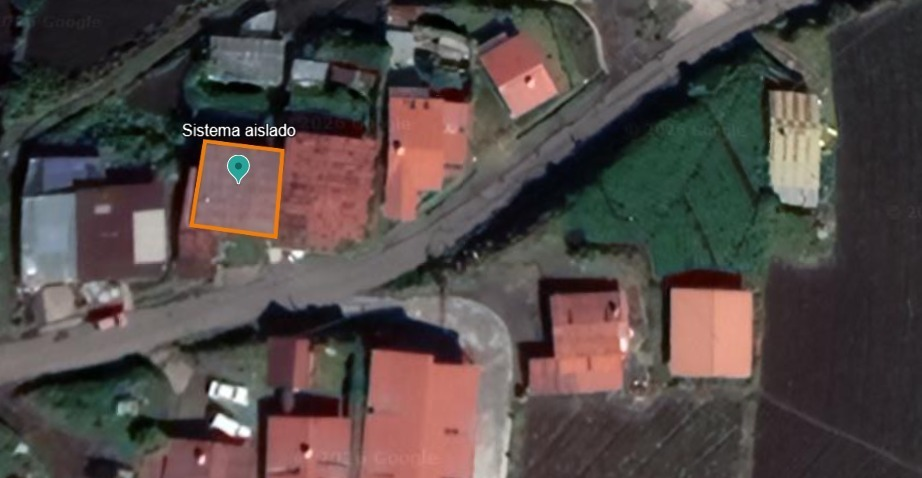
\includegraphics[width=\anchofig]{ubicacion_satelital.jpg}
\caption{Ubicación de la vivienda en Santa Rosa de Oreamuno (imagen de Google Earth). El recuadro marca el techo.}
\label{fig:satelital}
\end{figure}

El sitio está en las faldas del volcán Irazú, a \SI{2317}{m} de altura, en una zona de viviendas rodeada de terrenos de cultivo, como se observa en la Fig.~\ref{fig:satelital}. Por la altura, el clima es frío: en los últimos doce meses la temperatura varió entre 7 y \SI{29.5}{\celsius}. La temperatura media mensual de PVGIS está entre 16.3 y \SI{18.6}{\celsius} (Sección~\ref{sec:recurso}). En la imagen satelital no se identifican edificaciones ni árboles más altos junto a la cara este del techo; la ausencia de sombras debe confirmarse en el sitio.

El techo es de lámina de zinc ondulada, a dos aguas, con la cumbrera en dirección norte--sur, de modo que una cara mira al este y la otra al oeste, ambas con \SI{12}{\degree} de inclinación. En planta mide unos \SI{85}{m^2}, aproximadamente \SI{9.2}{m} por lado, de modo que cada cara tiene unos \SI{4.6}{m} de ancho horizontal (\SI{4.7}{m} sobre la pendiente) y \SI{9.2}{m} de largo.

\subsection{Caracterización del consumo}

\subsubsection{Cargas críticas}

Se levantó la lista de los equipos de la casa con sus horas de uso y se tomaron los datos de placa de los principales. Con el dueño se definieron como cargas críticas las que deben seguir funcionando si falla el servicio: la refrigeración de alimentos, la iluminación y las comunicaciones. Quedaron fuera la ducha eléctrica, la cocina, el microondas, la lavadora y la cámara de refrigeración. La Tabla~\ref{tab:cargas} presenta las cargas críticas y la Fig.~\ref{fig:consumo_equipos}, su energía diaria.

\begin{table*}[!htb]
\caption{Cargas críticas de la vivienda}
\label{tab:cargas}
\centering
\footnotesize
\setlength{\tabcolsep}{3pt}
\begin{tabular}{l c c c c c c c r}
\toprule
Equipo & Cant. & $V$ [V] & $P_{\mathrm{nom}}$ [W] & $P_{\mathrm{pico}}$ [W] & $I_{\mathrm{nom}}$ [A] & $I_{\max}$ [A] & Horas/día & Energía [Wh/día] \\
\midrule
Refrigerador Atlas AC12SSAAWA & 1 & 115 & 196.7 & 786.8\textsuperscript{a} & 1.71 & 6.84\textsuperscript{a} & 9 & 1770.3 \\
Congelador Daytron MCHF90 & 1 & 115 & 130.0 & 520.0\textsuperscript{a} & 1.20 & 4.80\textsuperscript{a} & 10 & 1300.0 \\
Cargadores de celular (5)\textsuperscript{b} & 1 & 120 & 35.0 & 175.0 & 0.29 & 1.46 & 12 & 420.0 \\
Cargadores de laptop (3)\textsuperscript{c} & 1 & 120 & 51.7 & 155.1 & 0.43 & 1.29 & 6 & 310.2 \\
Bombillos LED Sylvania A60 & 3 & 120 & 15.0 & 15.0 & 0.13 & 0.13 & 5 & 225.0 \\
Bombillos LED Sylvania A60 & 4 & 120 & 15.0 & 15.0 & 0.13 & 0.13 & 2 & 120.0 \\
Bombillo LED Sylvania A60 & 1 & 120 & 15.0 & 15.0 & 0.13 & 0.13 & 3 & 45.0 \\
Módem Nexxt Nebula N300 & 1 & 120 & 6.0 & 6.0 & 0.05 & 0.05 & 24 & 144.0 \\
\midrule
\multicolumn{8}{l}{Total (todas las cargas en CA, 120 V)} & 4334.5 \\
\bottomrule
\end{tabular}
\\[2pt]
{\footnotesize Datos de placa y de la lista de equipos (noviembre de 2026). Donde la placa no da la tensión se usa \SI{120}{V}, y la corriente se calcula como $P/V$.
\textsuperscript{a}Supuesto: arranque del compresor de 4 veces la potencia nominal, el valor alto del intervalo típico de 3 a 4 veces.
\textsuperscript{b}Cargadores de 40, 35, 35, 45 y \SI{20}{W}; se usa la potencia media de \SI{35}{W} con 12 horas de carga en total, y como pico los cinco a la vez (\SI{175}{W}).
\textsuperscript{c}Delta de \SI{45.1}{W}, Lenovo de \SI{65.0}{W} y HP de \SI{45.0}{W}; potencia media de \SI{51.7}{W} con 6 horas en total, y como pico los tres a la vez.}
\end{table*}

\begin{figure}[!htb]
\centering
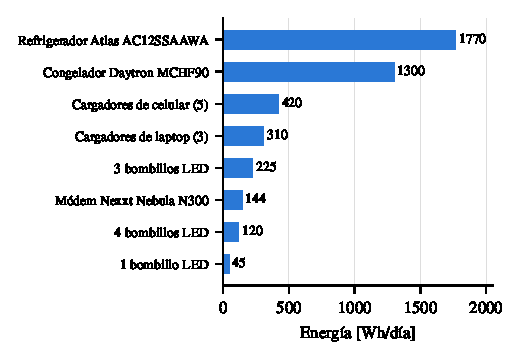
\includegraphics[width=\anchofig]{consumo_equipos.pdf}
\caption{Energía diaria de las cargas críticas.}
\label{fig:consumo_equipos}
\end{figure}

Las cargas críticas consumen \SI{4334.5}{Wh} por día, todas en corriente alterna a \SI{120}{V}. El refrigerador y el congelador suman \SI{3070}{Wh}, el 71\,\% del total. Si todas las cargas se encienden a la vez, incluidos los cinco cargadores de celular y los tres de laptop, la potencia es de \SI{783}{W}; si además arrancan los dos compresores, el pico llega a \SI{1763}{W}. Estos dos valores se usan para seleccionar el inversor.

\subsubsection{Consumo de la vivienda}

Se cuenta con la factura de JASEC de octubre de 2026, por ¢19\,175, y se sabe que las facturas han estado entre ¢16\,000 y ¢22\,000. Con la tarifa residencial de JASEC para 2026 \cite{aresep_tre}, el alumbrado público \cite{aresep_ap}, el tributo de bomberos (1.75\,\% del cargo de energía cuando se superan \SI{100}{kWh}) \cite{ley8992} y el IVA (13\,\% del cargo de energía cuando se superan \SI{280}{kWh}) \cite{ley9635}, la factura de octubre corresponde a \SI{275}{kWh}. La Tabla~\ref{tab:tarifa} resume la tarifa.

\begin{table}[!htb]
\caption{Tarifa residencial de JASEC (T-RE) para 2026}
\label{tab:tarifa}
\centering
\footnotesize
\begin{tabular}{l r}
\toprule
Cargo & Valor \\
\midrule
Energía, primeros \SI{30}{kWh} (cargo fijo) & ¢1863.30 \\
Energía, de 31 a \SI{200}{kWh} & ¢62.11/kWh \\
Energía, más de \SI{200}{kWh} & ¢76.02/kWh \\
Alumbrado público, primeros \SI{30}{kWh} & ¢80.10 \\
Alumbrado público, más de \SI{30}{kWh} & ¢2.67/kWh \\
Bomberos (más de \SI{100}{kWh}) & 1.75\,\% del cargo de energía \\
IVA (más de \SI{280}{kWh}) & 13\,\% del cargo de energía \\
\bottomrule
\end{tabular}
\\[2pt]
{\footnotesize Las facturas se redondean al múltiplo de ¢5 más cercano.}
\end{table}

Como solo se tiene una factura, los demás meses se estimaron con la variación mensual de un ejemplo de facturación de una vivienda servida por JASEC: los meses que en el ejemplo superan a octubre conservan la misma proporción, y en los que quedan por debajo la diferencia con octubre se redujo para que el mes más bajo diera unos ¢16\,100. Diciembre, que es el mes de mayor consumo de la casa, se igualó al mes más alto del resto del año. El resultado está en la Tabla~\ref{tab:facturas} y en la Fig.~\ref{fig:facturas}: \SI{3230}{kWh} y ¢236\,730 al año, con facturas de ¢16\,135 a ¢22\,495. Las cargas críticas representan el 49\,\% del consumo anual de la casa.

\begin{table}[!htb]
\caption{Consumo y factura mensual estimados para 2026}
\label{tab:facturas}
\centering
\footnotesize
\setlength{\tabcolsep}{4pt}
\begin{tabular}{l r r r r}
\toprule
Mes & Casa [kWh] & Cargas críticas [kWh] & Factura actual [¢] & Factura con el sistema [¢] \\
\midrule
Ene & 237.0 & 134.4 & 16\,135 & 6\,760 \\
Feb & 256.1 & 121.4 & 17\,665 & 8\,875 \\
Mar & 281.0 & 134.4 & 22\,070 & 9\,660 \\
Abr & 257.8 & 130.0 & 17\,800 & 8\,415 \\
May & 276.3 & 134.4 & 19\,280 & 9\,350 \\
Jun & 283.7 & 130.0 & 22\,315 & 10\,120 \\
Jul & 241.4 & 134.4 & 16\,485 & 7\,050 \\
Ago & 285.7 & 134.4 & 22\,495 & 9\,970 \\
Set & 281.9 & 130.0 & 22\,150 & 10\,005 \\
Oct\textsuperscript{a} & 275.0 & 134.4 & 19\,175 & 9\,265 \\
Nov & 268.6 & 130.0 & 18\,665 & 9\,125 \\
Dic & 285.7 & 134.4 & 22\,495 & 9\,970 \\
\midrule
Total & 3230.2 & 1582.1 & 236\,730 & 108\,565 \\
\bottomrule
\end{tabular}
\\[2pt]
{\footnotesize \textsuperscript{a}Factura real. Los demás meses son estimados. La factura con el sistema se explica en la Sección~\ref{sec:economia}.}
\end{table}

\begin{figure}[!htb]
\centering
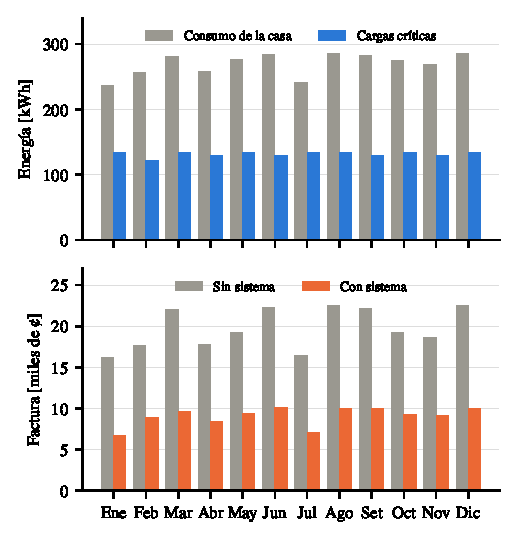
\includegraphics[width=\anchofig]{consumo_facturas.pdf}
\caption{Consumo mensual de la casa y de las cargas críticas (arriba) y factura sin y con el sistema (abajo).}
\label{fig:facturas}
\end{figure}
